\documentclass[12pt,a4paper]{article}

% ─── Page Layout ───────────────────────────────────────────────────────────────
\usepackage[a4paper, margin=0.8in, headheight=14pt]{geometry}

% ─── Fonts (XeLaTeX) ───────────────────────────────────────────────────────────
\usepackage{fontspec}
\usepackage{unicode-math}
\setmainfont{TeX Gyre Pagella}
\setmonofont[Scale=0.88]{TeX Gyre Cursor}
\setmathfont{Latin Modern Math}

% ─── Packages ──────────────────────────────────────────────────────────────────
\usepackage{xcolor}
\usepackage{colortbl}
\usepackage{titlesec}
\usepackage{enumitem}
\usepackage{tabularx}
\usepackage{booktabs}
\usepackage{array}
\usepackage{amsmath}
\usepackage{tikz}
\usetikzlibrary{shapes.geometric, arrows.meta, positioning, calc, fit, decorations.pathreplacing, patterns}
\usepackage{tcolorbox}
\tcbuselibrary{skins, breakable}
\usepackage{hyperref}
\usepackage{fancyhdr}
\usepackage{graphicx}
\usepackage{microtype}
\hyphenpenalty=10000
\exhyphenpenalty=10000
\sloppy
\usepackage{caption}
\usepackage{setspace}
\usepackage{multirow}
\usepackage{tocloft}

% ─── Q&A helper ────────────────────────────────────────────────────────────────
\newcommand{\Q}[1]{\textbf{#1}\par\noindent\ignorespaces}

% ─── Colour Palette ────────────────────────────────────────────────────────────
\definecolor{myred}{RGB}{196,30,58}
\definecolor{mydark}{RGB}{30,30,50}
\definecolor{mygreen}{RGB}{14,120,80}
\definecolor{myteal}{RGB}{0,130,140}
\definecolor{myamber}{RGB}{180,100,0}
\definecolor{mypurple}{RGB}{100,30,160}
\definecolor{mygray}{RGB}{246,247,249}
\definecolor{mgframe}{RGB}{180,185,200}
\definecolor{watermark}{RGB}{145,150,170}
\definecolor{hdrred}{RGB}{250,232,235}
\definecolor{hdrgreen}{RGB}{220,244,233}
\definecolor{hdrteal}{RGB}{220,242,244}
\definecolor{hdramber}{RGB}{253,242,215}
\definecolor{hdrpurple}{RGB}{238,228,255}
\definecolor{hdrgray}{RGB}{238,240,245}
\definecolor{rowalt}{RGB}{250,251,253}

% ─── Section Formatting ────────────────────────────────────────────────────────
\titleformat{\section}
  {\large\bfseries\color{myred}}{\thesection.}{0.5em}{}
  [\vspace{1pt}{\color{myred}\rule{\linewidth}{0.8pt}}]
\titleformat{\subsection}
  {\normalsize\bfseries\color{myteal}}{\thesubsection}{0.5em}{}
\titlespacing*{\section}{0pt}{18pt}{7pt}
\titlespacing*{\subsection}{0pt}{11pt}{4pt}

% ─── Paragraph ─────────────────────────────────────────────────────────────────
\setlength{\parindent}{0pt}
\setlength{\parskip}{4pt}

% ─── TOC Styling ───────────────────────────────────────────────────────────────
\renewcommand{\cfttoctitlefont}{\large\bfseries\color{myred}}
\renewcommand{\cftaftertoctitle}{\par\noindent{\color{myred}\rule{\linewidth}{0.8pt}}}
\setlength{\cftbeforetoctitleskip}{0pt}
\setlength{\cftaftertoctitleskip}{6pt}
\renewcommand{\cftsecfont}{\normalsize\bfseries\color{mydark}}
\renewcommand{\cftsecpagefont}{\normalsize\bfseries\color{mydark}}
\renewcommand{\cftsecleader}{\cftdotfill{\cftdotsep}}
\setlength{\cftbeforesecskip}{7pt}
\renewcommand{\cftsubsecfont}{\small\color{mydark}}
\renewcommand{\cftsubsecpagefont}{\small\color{mydark}}
\setlength{\cftbeforesubsecskip}{3pt}
\setlength{\cftsubsecindent}{1.4em}

% ─── Table helpers ─────────────────────────────────────────────────────────────
\renewcommand{\arraystretch}{1.45}
\setlength{\tabcolsep}{6pt}
\arrayrulecolor{mydark}
\newcolumntype{B}[1]{>{\small\bfseries\raggedright\arraybackslash}m{#1}}
\newcolumntype{Y}{>{\small\raggedright\arraybackslash}X}
\renewcommand{\tabularxcolumn}[1]{m{#1}}

% ─── Header / Footer ───────────────────────────────────────────────────────────
\pagestyle{fancy}
\fancyhf{}
\fancyhead[L]{\small\color{myred}\textbf{EC401}\;\color{mydark}--- Analog Communication}
\fancyhead[R]{\small\color{myteal}\textbf{Module 1 Notes}}
\fancyfoot[C]{\small\color{mydark}\thepage}
\fancyfoot[R]{\small\color{watermark}\textit{\copyright\ Biraj}}
\renewcommand{\headrulewidth}{0.5pt}
\renewcommand{\footrulewidth}{0.3pt}

% ─── Hyperref ──────────────────────────────────────────────────────────────────
\hypersetup{
  colorlinks=true, linkcolor=myteal, urlcolor=myteal,
  pdfauthor={Biraj Sarkar (CGEC)},
  pdftitle={EC401 --- Module 1 Notes: Introduction and Continuous Wave Linear Modulation}
}

% ─── tcolorbox styles ──────────────────────────────────────────────────────────
\tcbset{
  tikzbox/.style={
    colback=mygray, colframe=mgframe, boxrule=0.6pt, arc=4pt,
    left=8pt, right=8pt, top=6pt, bottom=6pt,
    colbacktitle=mgframe, coltitle=mydark, fonttitle=\small\bfseries
  },
  defbox/.style={
    colback=hdrgreen, colframe=mygreen, boxrule=0.8pt, arc=4pt,
    left=9pt, right=9pt, top=6pt, bottom=6pt,
    colbacktitle=mygreen, coltitle=white, fonttitle=\small\bfseries
  },
  formulabox/.style={
    colback=hdrteal, colframe=myteal, boxrule=0.8pt, arc=4pt,
    left=9pt, right=9pt, top=7pt, bottom=7pt,
    colbacktitle=myteal, coltitle=white, fonttitle=\small\bfseries
  },
  examplebox/.style={
    colback=hdramber, colframe=myamber, boxrule=0.8pt, arc=4pt,
    left=9pt, right=9pt, top=6pt, bottom=6pt,
    colbacktitle=myamber, coltitle=white, fonttitle=\small\bfseries
  },
  masonbox/.style={
    colback=hdrpurple, colframe=mypurple, boxrule=0.8pt, arc=4pt,
    left=9pt, right=9pt, top=6pt, bottom=6pt,
    colbacktitle=mypurple, coltitle=white, fonttitle=\small\bfseries
  },
  exambox/.style={
    colback=hdrpurple, colframe=mypurple, boxrule=1pt, arc=5pt,
    left=10pt, right=10pt, top=8pt, bottom=8pt,
    colbacktitle=mypurple, coltitle=white, fonttitle=\bfseries,
    breakable, title after break={\textbf{Frequently Asked / Viva Questions (contd.)}}
  }
}
% Allow all boxes to break across pages — prevents footer overflow
\tcbset{breakable}
\tcbset{after={\color{black}}}

% ─── TikZ styles ───────────────────────────────────────────────────────────────
\tikzset{
  block/.style={rectangle, draw=myteal, fill=hdrteal,
    text width=2.4cm, align=center, minimum height=0.95cm,
    font=\small, rounded corners=3pt, line width=0.7pt},
  redblock/.style={rectangle, draw=myred, fill=hdrred,
    text width=2.4cm, align=center, minimum height=0.95cm,
    font=\small, rounded corners=3pt, line width=0.7pt},
  netnode/.style={rectangle, draw=myteal, fill=hdrteal,
    text width=1.5cm, align=center, minimum height=0.8cm,
    font=\small, rounded corners=3pt, line width=0.7pt},
  sumjunc/.style={circle, draw=myamber, fill=hdramber,
    minimum size=0.62cm, font=\small, line width=0.8pt},
  snode/.style={circle, draw=mypurple, fill=hdrpurple,
    minimum size=0.55cm, font=\footnotesize, line width=0.7pt},
  arrow/.style={-Stealth, thick, color=mydark},
  redarrow/.style={-Stealth, thick, color=myred},
  line/.style={thick, color=mydark}
  % ⚠ Do NOT define axis/.style here — conflicts with pgfplots/library keys.
  %   Use inline style instead: \draw[-Stealth, thin, color=mydark]
}

\begin{document}

% ─── Title Page ───────────────────────────────────────────────────────────────
\begin{center}
  {\LARGE\bfseries\color{myred} EC401 --- Analog Communication}\\[5pt]
  {\normalsize\color{mydark} Semester IV \quad$\bullet$\quad 3L:0T:0P \quad$\bullet$\quad 3 Credits}\\[3pt]
  {\normalsize\color{myteal}\textbf{Module 1 Exam Notes: Introduction and Continuous Wave Linear Modulation}}\\[3pt]
  {\small\color{mydark} CGEC \;$|$\; B.Tech ECE (2023--27) \;$|$\; \textit{Biraj Sarkar}}
\end{center}
\vspace{2pt}
\noindent{\color{myred}\rule{\linewidth}{1.5pt}}
\vspace{2pt}

\hypersetup{linkcolor=mydark}
\tableofcontents
\hypersetup{linkcolor=myteal}
\newpage

\section{Introduction to Analog Communication}

\begin{tcolorbox}[defbox, title={Communication System and Modulation}]
An analog communication system carries a continuously varying message from source to destination. The transmitter converts the message to a suitable electrical waveform, modulates a carrier and provides power for transmission. The channel (free space, cable or another medium) introduces attenuation, distortion and noise. The receiver selects and amplifies the desired signal, demodulates it and drives the output transducer.
\end{tcolorbox}

\begin{tcolorbox}[tikzbox, unbreakable, title={Transmitter, Channel and Receiver}]
\centering
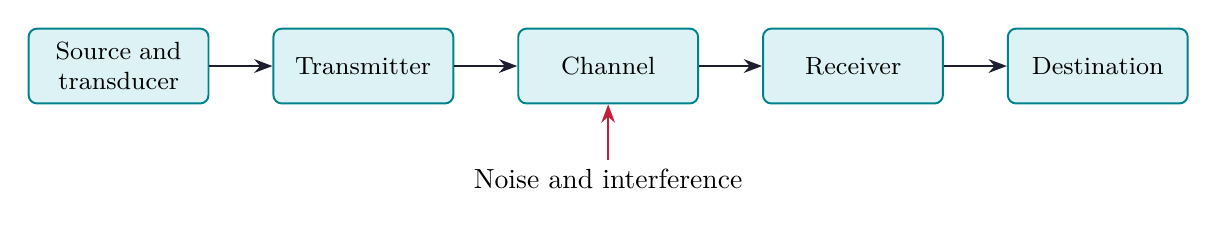
\begin{tikzpicture}[node distance=8mm,sblock/.style={block,text width=2.05cm}]
  \node[sblock] (src) {Source and transducer};
  \node[sblock,right=of src] (tx) {Transmitter};
  \node[sblock,right=of tx] (ch) {Channel};
  \node[sblock,right=of ch] (rx) {Receiver};
  \node[sblock,right=of rx] (dst) {Destination};
  \draw[arrow] (src)--(tx);
  \draw[arrow] (tx)--(ch);
  \draw[arrow] (ch)--(rx);
  \draw[arrow] (rx)--(dst);
  \node[below=7mm of ch] (noise) {Noise and interference};
  \draw[redarrow] (noise)--(ch);
\end{tikzpicture}\par
\end{tcolorbox}

Modulation varies a carrier parameter according to the message. It makes antennas practical, fits signals to a channel passband and separates simultaneous transmissions by frequency. In amplitude modulation the message varies one or both carrier amplitude components. In angle modulation information varies phase or instantaneous frequency.

\subsection{Baseband, Passband and Channel Selection}
A microphone or sensor usually produces a \textbf{baseband} waveform whose useful frequencies extend from near DC to $W$. The transmitter chooses a sinusoidal carrier in the allocated band and translates the message around it. A channel of usable RF bandwidth $B_{\rm ch}$ must pass the resulting spectrum. An RF filter at the receiver selects the channel before demodulation. The recovered audio is then selected by a baseband low-pass filter.

\begin{tcolorbox}[formulabox, title={Why Carrier Multiplication Shifts the Spectrum}]
For $\mathcal F\{m(t)\}=M(f)$ and angular frequency $\omega_c=2\pi f_c$,
\[
\begin{aligned}
 m(t)\cos\omega_ct
   &=\tfrac12m(t)e^{j\omega_ct}+\tfrac12m(t)e^{-j\omega_ct},\\
 \mathcal F\{m(t)\cos\omega_ct\}
   &=\tfrac12M(f-f_c)+\tfrac12M(f+f_c).
\end{aligned}
\]
The positive-frequency copy lies between $f_c-W$ and $f_c+W$. For example, a message limited to $4\,\mathrm{kHz}$ sent on a $200\,\mathrm{kHz}$ carrier occupies $196$--$204\,\mathrm{kHz}$ before any guard bands are added. Its negative-frequency mirror is required because the time waveform is real.
\end{tcolorbox}

A nearly flat gain and approximately linear phase over the occupied band preserve the waveform shape up to gain and delay. A selective notch inside a sideband removes particular message components. This is why frequency allocation, channel selectivity and modulation bandwidth have to be considered together.

\begin{tcolorbox}[examplebox, title={Quarter-Wave Antenna Length}]
With $c\approx3\times10^8\,\mathrm{m/s}$,
\[
\begin{aligned}
 \ell&=\lambda/4=c/(4f),\\
 \ell_{5\,\mathrm{kHz}}&=\frac{3\times10^8}{4(5\times10^3)}\,\mathrm{m}
     =15\,\mathrm{km},\\
 \ell_{1\,\mathrm{MHz}}&=\frac{3\times10^8}{4(10^6)}\,\mathrm{m}
     =75\,\mathrm{m}.
\end{aligned}
\]
\end{tcolorbox}

\section{Conventional AM with Transmitted Carrier}
The transmitter sends a carrier alongside two shifted versions of the message. This allows a simple receiver to recover the audio from the envelope.

\subsection{Time-Domain Expression and Envelope}

\begin{tcolorbox}[defbox, title={Double Sideband with Transmitted Carrier (DSB-TC)}]
For carrier peak $A_c$ in volts, carrier frequency $f_c$ in hertz and sensitivity $k_a$ in $\mathrm{V^{-1}}$,
\[
s(t)=A_c[1+k_a m(t)]\cos(2\pi f_ct).
\]
For a tone $m(t)=A_m\cos(2\pi f_mt)$, $\mu=k_aA_m$ is the dimensionless modulation index. The signed envelope factor is $1+\mu\cos(2\pi f_mt)$.
\end{tcolorbox}

Using $\cos a\cos b=\tfrac12[\cos(a+b)+\cos(a-b)]$,
\[
\begin{aligned}
 s(t)&=A_c\cos(2\pi f_ct)+\mu A_c\cos(2\pi f_mt)\cos(2\pi f_ct)\\
     &=A_c\cos(2\pi f_ct)\\
     &\quad+\frac{\mu A_c}{2}\cos[2\pi(f_c+f_m)t]\\
     &\quad+\frac{\mu A_c}{2}\cos[2\pi(f_c-f_m)t].
\end{aligned}
\]
The upper and lower sidebands (USB and LSB) are at $f_c+f_m$ and $f_c-f_m$. Each has peak voltage $\mu A_c/2$.

\subsection{Spectrum and Bandwidth}
With the transform kernel $e^{-j2\pi ft}$, a cosine of peak $A$ contributes two impulses of weight $A/2$. With $M(f)$ supported on $|f|\le W$,
\[
\begin{aligned}
 S(f)&=\frac{A_c}{2}[\delta(f-f_c)+\delta(f+f_c)]\\
     &\quad+\frac{k_a A_c}{2}[M(f-f_c)+M(f+f_c)],\\
 B_{\mathrm{AM}}&=(f_c+W)-(f_c-W)=2W\quad(\mathrm{Hz}).
\end{aligned}
\]
For a tone the carrier impulses have weight $A_c/2$ each, and the four sideband impulses have weight $\mu A_c/4$ each.

\begin{tcolorbox}[tikzbox, unbreakable, title={Two-Sided Spectrum of Single-Tone AM}]
\centering
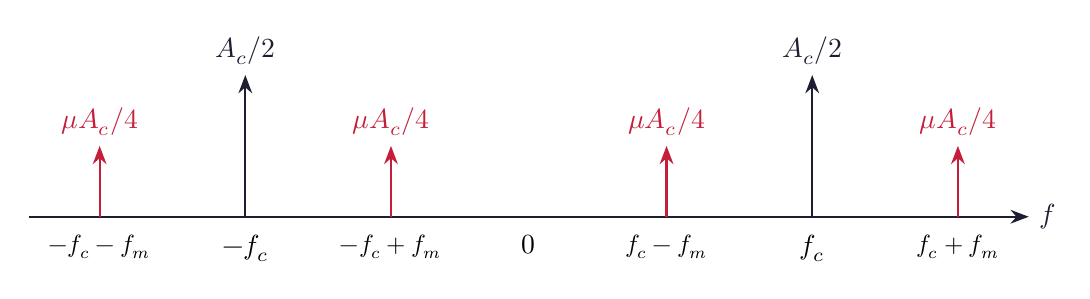
\begin{tikzpicture}
 \draw[arrow] (-6.35,0)--(6.35,0) node[right] {$f$};
 \node[below=3pt] at (0,0) {$0$};
 \foreach \x/\ff in {-3.6/-f_c,3.6/f_c}{
   \draw[arrow] (\x,0)--(\x,1.8) node[above] {$A_c/2$};
   \node[below=3pt] at (\x,0) {$\ff$};
 }
 \foreach \x/\ff in {-5.45/-f_c-f_m,-1.75/-f_c+f_m,1.75/f_c-f_m,5.45/f_c+f_m}{
   \draw[redarrow] (\x,0)--(\x,0.9) node[above] {$\mu A_c/4$};
   \node[below=3pt] at (\x,0) {\small $\ff$};
 }
\end{tikzpicture}\par
\end{tcolorbox}

\subsection{Carrier-Referenced Phasors}
In a frame rotating at $2\pi f_c$, the carrier is stationary. The USB and LSB rotate in opposite directions at $2\pi f_m$. Their transverse components cancel. Their horizontal components add to $\mu A_c\cos(2\pi f_mt)$.

\begin{tcolorbox}[tikzbox, unbreakable, title={AM Phasors at a Representative Instant}]
\centering
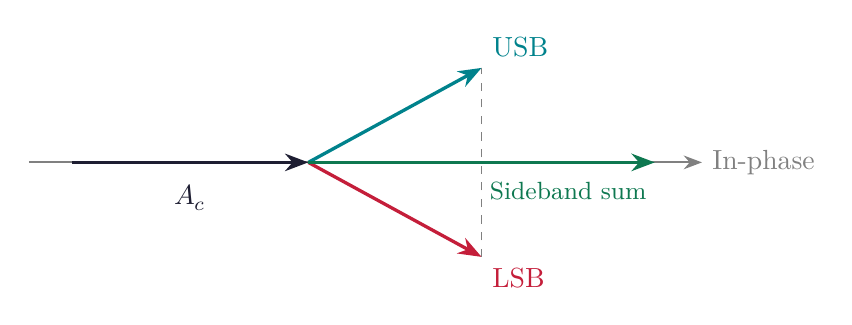
\begin{tikzpicture}
 \draw[arrow,gray] (-0.55,0)--(8.0,0) node[right] {In-phase};
 \draw[arrow,very thick] (0,0)--(3,0) node[midway,below=4pt] {$A_c$};
 \draw[arrow,myteal,very thick] (3,0)--(5.2,1.2) node[above right] {USB};
 \draw[redarrow,very thick] (3,0)--(5.2,-1.2) node[below right] {LSB};
 \draw[dashed,gray] (5.2,-1.2)--(5.2,1.2);
 \draw[arrow,mygreen,very thick] (3,0)--(7.4,0);
 \node[mygreen,below] at (6.3,-0.12) {\small Sideband sum};
\end{tikzpicture}\par
\small Both sideband vectors have magnitude $\mu A_c/2$. Their projections add to the in-phase carrier.
\end{tcolorbox}

\subsection{Under-, Critical and Overmodulation}
The magnitude envelope is $A_c|1+\mu\cos(2\pi f_mt)|$. For $\mu<1$ it stays positive. At $\mu=1$ it touches zero. For $\mu>1$ the signed factor becomes negative near the trough, reversing RF phase by $\pi$. Envelope detection folds this interval, causing distortion.

\begin{tcolorbox}[tikzbox, unbreakable, title={Signed Envelope Factor at Three Modulation Depths}]
\centering
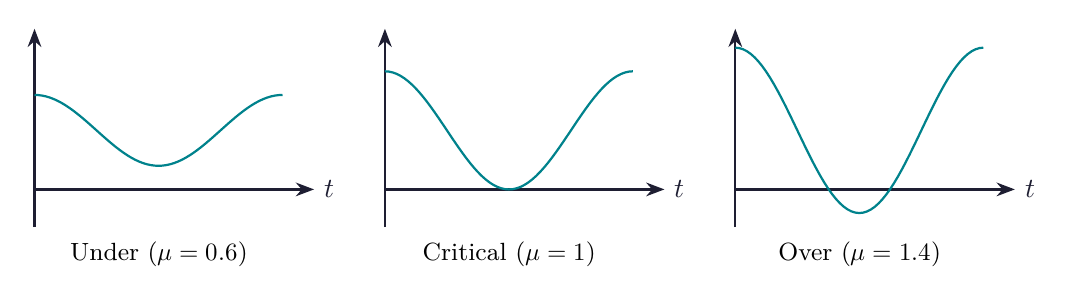
\begin{tikzpicture}
 \foreach \offset/\depth/\label in {0/0.6/Under,4.45/1/Critical,8.9/1.4/Over}{
   \begin{scope}[shift={(\offset,0)}]
    \draw[arrow] (0,0)--(3.55,0) node[right] {$t$};
    \draw[arrow] (0,-0.48)--(0,2.04);
    \draw[myteal,thick,domain=0:3.15,samples=65]
      plot (\x,{0.75*(1+\depth*cos(360*\x/3.15))});
    \node[below] at (1.58,-0.54) {\small \label\ ($\mu=\depth$)};
   \end{scope}
 }
\end{tikzpicture}\par
\end{tcolorbox}

For a nonfolded envelope,
\[
\begin{aligned}
 E_{\max}-E_{\min}&=2A_c\mu,\\
 E_{\max}+E_{\min}&=2A_c,\\
 \mu&=\frac{E_{\max}-E_{\min}}{E_{\max}+E_{\min}}.
\end{aligned}
\]

\subsection{Transmitted Power and Efficiency}
Across a resistance $R$ in ohms, a tone of peak $A$ delivers $A^2/(2R)$ watts. Power at distinct frequencies adds after time averaging.
\begin{tcolorbox}[formulabox, title={Power of Single-Tone AM}]
\[
\begin{aligned}
 P_c &= \frac{A_c^2}{2R},\\
 P_{\mathrm{USB}}=P_{\mathrm{LSB}}&=\frac{(\mu A_c/2)^2}{2R}
                                  =\frac{\mu^2}{4}P_c,\\
 P_{\mathrm{SB}}&=\frac{\mu^2}{2}P_c,\qquad P_T=P_c+P_{\mathrm{SB}},\\
 \eta&=\frac{P_{\mathrm{SB}}}{P_T}=\frac{\mu^2}{2+\mu^2}.
\end{aligned}
\]
Critical single-tone AM has $\eta=1/3$. The carrier simplifies envelope reception but does not carry message variation.
\end{tcolorbox}

\begin{tcolorbox}[examplebox, title={Identify AM Frequencies and Calculate Power}]
For $s(t)=[20+12\cos(2\pi\,5000t)]\cos(2\pi\,100000t)$ and $R=50\,\Omega$, the index is $12/20=0.6$. The carrier is at $100\,\mathrm{kHz}$. Sidebands at $95$ and $105\,\mathrm{kHz}$ have peak $6\,\mathrm{V}$ each and span $10\,\mathrm{kHz}$.
\[
\begin{aligned}
 P_c&=\frac{20^2}{2(50)}=4\,\mathrm{W},\\
 P_{\mathrm{USB}}=P_{\mathrm{LSB}}&=\frac{6^2}{2(50)}=0.36\,\mathrm{W},\\
 P_T&=4+2(0.36)=4.72\,\mathrm{W},\\
 \eta&=\frac{0.72}{4.72}\approx15.25\%.
\end{aligned}
\]
\end{tcolorbox}

\subsection{Total Power for a General Zero-Mean Message}
Suppose $m(t)$ is zero mean, with mean-square value $P_m=\overline{m^2(t)}$ in $\mathrm{V^2}$. The RF voltage is $A_c[1+k_am(t)]\cos\omega_ct$. Using $\cos^2\omega_ct=(1+\cos2\omega_ct)/2$, the RF term near $2f_c$ averages to zero for a separated message band. The surviving terms give
\[
\begin{aligned}
 P_T &= \frac{A_c^2}{2R}\overline{[1+k_am(t)]^2}\\
     &= P_c[1+2k_a\overline{m(t)}+k_a^2P_m]\\
     &= P_c(1+k_a^2P_m),\\
 P_{\rm SB}&=P_c k_a^2P_m,\qquad
 \eta=\frac{k_a^2P_m}{1+k_a^2P_m}.
\end{aligned}
\]
For one tone $P_m=A_m^2/2$, so this reduces to the single-tone result. The $\mu=1$ efficiency limit quoted for one tone should be applied with that waveform assumption. Overmodulation depends on the most negative value of $1+k_am(t)$, which is a peak constraint.

\begin{tcolorbox}[examplebox, title={Two-Tone AM from Envelope Constraint to Transmitted Power}]
A $250\,\mathrm{kHz}$ carrier has $P_c=80\,\mathrm W$. Its signed envelope factor is
$1+0.5\cos(2\pi\,1000t)+0.3\cos(2\pi\,4000t)$.
\[
\begin{aligned}
 1+0.5\cos(2\pi\,1000t)+0.3\cos(2\pi\,4000t)&\ge 1-0.5-0.3=0.2,\\
 P_{\rm SB}&=80\left(\frac{0.5^2}{2}+\frac{0.3^2}{2}\right)
              =13.6\,\mathrm W,\\
 P_T&=80+13.6=93.6\,\mathrm W,\qquad
 \eta=\frac{13.6}{93.6}\approx14.5\%.
\end{aligned}
\]
The carrier and the four sidebands are at $250$, $249$, $251$, $246$ and $254\,\mathrm{kHz}$. Each $1\,\mathrm{kHz}$ sideband contributes $5\,\mathrm W$ and each $4\,\mathrm{kHz}$ sideband $1.8\,\mathrm W$. The positive lower bound proves there is no envelope folding. It need not be the actual minimum of the sum.
\end{tcolorbox}

\section{DSB-SC, SSB and Vestigial Sideband}
\subsection{Double Sideband Suppressed Carrier}
For dimensionless, zero-mean $m(t)$ of bandwidth $W$ and carrier scale $A_c$ in volts,
\[
\begin{aligned}
 s_D(t)&=A_c m(t)\cos(2\pi f_ct),\\
 S_D(f)&=\frac{A_c}{2}[M(f-f_c)+M(f+f_c)],\\
 B_D&=2W.
\end{aligned}
\]
For a tone of peak $A_m$, the two sideband peaks are $A_cA_m/2$, so
\[
 P_D=2\frac{(A_cA_m/2)^2}{2R}=\frac{A_c^2 A_m^2}{4R}.
\]
In general $P_D=A_c^2\overline{m^2(t)}/(2R)$ under the narrowband assumption. Suppressing the carrier saves power. A coherent receiver is needed to preserve the sign of $m(t)$.

\subsection{SSB-SC and SSB-TC}
The two AM sidebands contain redundant information for a real message. A filter can keep the USB or LSB alone. In the Hilbert form, with $\widehat m(t)$ the Hilbert transform of $m(t)$,
\[
 s_{\mathrm{U/L}}(t)=K[m(t)\cos(2\pi f_ct)\mp\widehat m(t)\sin(2\pi f_ct)].
\]
For a cosine, $\widehat m$ is a sine. The difference produces the upper frequency and the sum the lower frequency. The positive-frequency occupied band is $[f_c,f_c+W]$ for USB or $[f_c-W,f_c]$ for LSB. Real signals also have the negative-frequency mirror. SSB-TC inserts a line at $f_c$, increasing transmitted power without increasing bandwidth. The line can assist synchronization. With a sufficiently strong carrier approximate envelope detection is possible, but coherent recovery avoids quadrature envelope distortion.

\begin{tcolorbox}[examplebox, title={Compare DSB-SC and Filtered SSB for the Same Tone}]
A balanced modulator produces $s_D(t)=12\cos(2\pi\,3000t)\cos(2\pi\,120000t)$ across a $50\,\Omega$ load. The product expansion gives two equal $6\,\mathrm V$ peaks at $117$ and $123\,\mathrm{kHz}$.
\[
 \begin{aligned}
 P_D&=2\frac{6^2}{2(50)}=0.72\,\mathrm W,\\
 P_{\mathrm{USB}}&=\frac{6^2}{2(50)}=0.36\,\mathrm W,\\
 P_{\mathrm{USB+carrier}}&=0.36+\frac{10^2}{2(50)}
                      =1.36\,\mathrm W.
 \end{aligned}
\]
The last case adds a $10\,\mathrm V$ peak carrier at $120\,\mathrm{kHz}$. Keep peak volts, RMS volts and impulse weights separate. A message limited to $3\,\mathrm{kHz}$ requires $6\,\mathrm{kHz}$ in DSB or $3\,\mathrm{kHz}$ in SSB.
\end{tcolorbox}

\subsection{Vestigial Sideband}
VSB keeps one complete sideband and a fraction of the other. With a vestige extending $f_v$ hertz beyond the carrier into the other side, $B_{\mathrm{VSB}}\approx W+f_v$. The relaxed transition suits messages with strong low-frequency components such as analog TV video. For flat coherent recovery, the translated responses of the idealized real VSB filter add to a constant across baseband.

\begin{tcolorbox}[tikzbox, unbreakable, title={Positive-Frequency Occupancy of the Linear Modulation Schemes}]
\centering
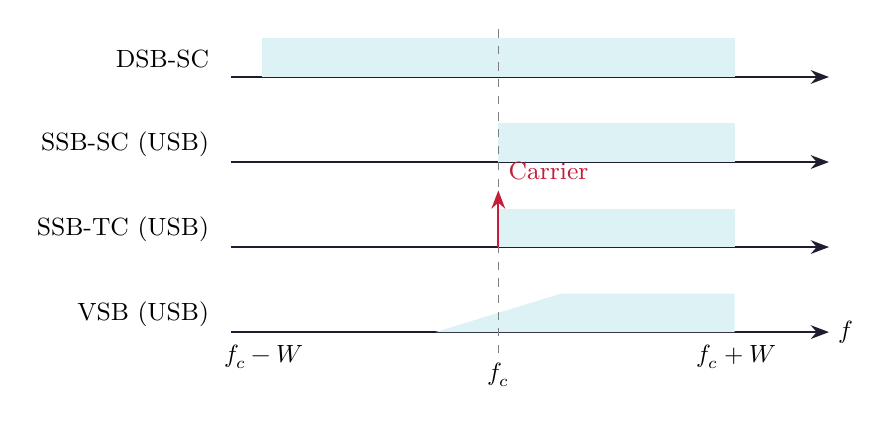
\begin{tikzpicture}[y=0.72cm,every node/.style={font=\small}]
 \foreach \y/\label in {5/DSB-SC,3.5/SSB-SC (USB),2/SSB-TC (USB),0.5/VSB (USB)}{
   \node[anchor=east] at (-3.55,\y+0.32) {\label};
   \draw[arrow] (-3.4,\y)--(4.2,\y);
 }
 \fill[hdrteal] (-3,5) rectangle (3,5.68);
 \fill[hdrteal] (0,3.5) rectangle (3,4.18);
 \fill[hdrteal] (0,2) rectangle (3,2.68);
 \fill[hdrteal] (-0.8,0.5)--(0.8,1.18)--(3,1.18)--(3,0.5)--cycle;
 \draw[dashed,gray] (0,0.13)--(0,5.86);
 \draw[redarrow] (0,2)--(0,3) node[above right] {\small Carrier};
 \node[below] at (-3,0.45) {$f_c-W$};
 \node[below] at (0,0.13) {$f_c$};
 \node[below] at (3,0.45) {$f_c+W$};
 \node[right] at (4.2,0.5) {$f$};
\end{tikzpicture}\par
\end{tcolorbox}


\subsection{Recovering the Baseband through a VSB Filter}
Consider the baseband-equivalent response of an ideal zero-phase RF filter. After filtering a DSB-SC signal, synchronous multiplication shifts the positive and negative RF bands back to baseband:
\[
\begin{aligned}
 S_D(f)&=\tfrac{A_c}{2}[M(f-f_c)+M(f+f_c)],\\
 Y(f)&=\tfrac{A_c}{2}M(f)\,[H(f+f_c)+H(f-f_c)],
       \qquad |f|\le W .
\end{aligned}
\]
This assumes a local oscillator of amplitude two and an ideal output low-pass filter. For a real, even response $H$, the two terms are $H(f_c+f)$ and $H(f_c-f)$. Their sum must be constant across the message band. Thus, near $f_c$, the decreasing response on one side complements the increasing response on the other. For unity target sum, $H(f_c)=1/2$. The spectrum sketch above shows occupied bands, while this condition explains why retaining a partial sideband can still give a flat recovered message.

\begin{tcolorbox}[examplebox, title={Check Complementary VSB Gain at Two Message Frequencies}]
Normalize the desired sum of the two VSB responses to one. At a $1\,\mathrm{kHz}$ offset, suppose the upper response is $0.82$ and the vestige response is $0.18$. At $3\,\mathrm{kHz}$ the full sideband has gain one and the vestige is zero.
\[
\begin{aligned}
 H(f_c+1\,\mathrm{kHz})+H(f_c-1\,\mathrm{kHz})&=0.82+0.18=1,\\
 H(f_c+3\,\mathrm{kHz})+H(f_c-3\,\mathrm{kHz})&=1+0=1.
\end{aligned}
\]
Both message components receive the same baseband gain $A_c/2$ in the chosen detector normalization. If the $1\,\mathrm{kHz}$ vestige is wrongly removed, that component falls to $0.82$ of its intended amplitude while the $3\,\mathrm{kHz}$ component stays the same.
\end{tcolorbox}

\newpage
\begin{center}
  {\large\bfseries\color{myred} Quick Revision --- Module 1}\\[3pt]
  {\small\color{mydark} Introduction and Continuous Wave Linear Modulation $|$ EC401}
\end{center}
\noindent{\color{myred}\rule{\linewidth}{1.2pt}}
\par\vspace{4pt}

\begin{tcolorbox}[formulabox, title={Key Formulas at a Glance}]
\renewcommand{\arraystretch}{1.35}
\noindent\begin{tabularx}{\linewidth}{B{4.4cm} Y}
Antenna length & $\ell=c/(4f)$ \\[4pt]
Conventional AM & $A_c(1+k_a m)\cos(2\pi f_ct)$ \\[4pt]
Tone sidebands & $f_c\pm f_m$, peak $\mu A_c/2$ each \\[4pt]
Envelope reading & $\mu=(E_{\max}-E_{\min})/(E_{\max}+E_{\min})$ \\[4pt]
Power and efficiency & $P_c=A_c^2/(2R)$ \newline $P_{\rm SB}=\mu^2P_c/2$ \quad $\eta=\mu^2/(2+\mu^2)$ \\[4pt]
DSB-SC power & $P_D=A_c^2\overline{m^2}/(2R)$ \\[4pt]
Bandwidth & DSB $2W$ \quad SSB $W$ \quad VSB $W+f_v$ \\[4pt]
\end{tabularx}\par
\end{tcolorbox}

\begin{tcolorbox}[defbox, title={One-Line Definitions}]
\begin{itemize}[leftmargin=*, itemsep=3pt, topsep=0pt]
  \item \textbf{Carrier.} A sinusoid used to position the message at RF.
  \item \textbf{Sideband.} A shifted part of the baseband spectrum carrying information.
  \item \textbf{Critical modulation.} The conventional AM envelope touches zero at $\mu=1$.
  \item \textbf{Vestige.} Part of the other sideband retained in VSB.
\end{itemize}
\end{tcolorbox}

\begin{tcolorbox}[exambox, title={Frequently Asked / Viva Questions}]
\begin{enumerate}[topsep=0pt, label=\textbf{Q\arabic*.}, itemsep=5pt]
  \item \Q{Why is modulation needed?}
    It enables practical antennas and places each signal in a suitable channel band.
  \item \Q{What do the transmitter and receiver do?}
    The transmitter prepares and launches the waveform. The receiver selects it and recovers the message.
  \item \Q{What are the AM lines for one tone?}
    $f_c$ and $f_c\pm f_m$, together with the negative-frequency mirrors.
  \item \Q{How do sideband phasors combine?}
    They rotate oppositely at $2\pi f_m$ in the carrier frame. In-phase projections add and transverse projections cancel.
  \item \Q{When is the envelope formula for modulation index valid?}
    When the magnitude envelope has no folding.
  \item \Q{What causes overmodulation distortion?}
    Negative portions of the signed envelope reverse RF phase. A magnitude detector folds them.
  \item \Q{What is the maximum single-tone conventional AM efficiency?}
    $1/3$ at $\mu=1$ for a nonfolded envelope.
  \item \Q{Why is DSB-SC received coherently?}
    The local reference preserves the sign of the message, which is lost in a magnitude detector.
  \item \Q{Does a transmitted SSB carrier increase bandwidth?}
    No. It adds a line at the existing band edge and increases power.
  \item \Q{Why is VSB useful near the carrier?}
    It relaxes the sharp transition required for SSB while keeping the bandwidth below full DSB.
\end{enumerate}
\end{tcolorbox}

\begin{tcolorbox}[tikzbox, unbreakable, title={Summary Comparison}]
\begingroup
\setlength{\tabcolsep}{5pt}
\setlength{\extrarowheight}{3pt}
\renewcommand{\arraystretch}{1.45}
\noindent\begin{tabularx}{\linewidth}{|B{3.35cm}|Y|Y|}
\hline
\multicolumn{1}{|c|}{\textbf{Scheme}} & \multicolumn{1}{c|}{\textbf{Transmitted components}} & \multicolumn{1}{c|}{\textbf{Bandwidth and use}} \\
\hline
DSB-TC & Carrier and both sidebands. & $2W$. Simple AM broadcast receivers. \\
\hline
DSB-SC & Both sidebands. & $2W$. Coherent reception. \\
\hline
SSB & One sideband, carrier optional. & $W$. Narrow voice channels. \\
\hline
VSB & Full sideband and vestige. & $W+f_v$. Analog video transmission. \\
\hline
\end{tabularx}\par
\endgroup
\end{tcolorbox}

\end{document}
